\section{Auswertung}
\label{sec:Auswertung}


\begin{table}[H]
    \centering
    \caption{Messwerte zur Bestimmung der Filterkurve.}
    \label{tab:filter}
    \begin{tabular}{c c}
        \toprule
        $\nu /kHz$ & $U / mV$ \\
        \midrule
        20    &  40   \\
        21    &  44   \\
        22    &  50   \\
        23    &  56   \\
        24    &  60   \\
        25    &  68   \\
        26    &  75   \\
        27    &  90   \\
        28    &  105  \\
        29    &  125  \\
        30    &  150  \\
        31    &  200  \\
        32    &  260  \\
        32.5  &  330  \\    
        33    &  440  \\
        33.3  &  500  \\ 
        33.5  &  600  \\
        33.8  &  700  \\
        34    &  800  \\
        34.3  &  1100  \\
        34.5  &  1300 \\
        34.8  &  1500 \\
        35    &  1400 \\
        35.3  &  1100 \\
        35.6  &  800 \\ 
        36    &  600 \\
        36.5  &  480 \\ 
        37    &  400 \\
        38    &  250 \\
        39    &  200 \\
        40    &  170 \\
        \bottomrule
    \end{tabular}
\end{table}



\begin{figure}[H]
    \centering
    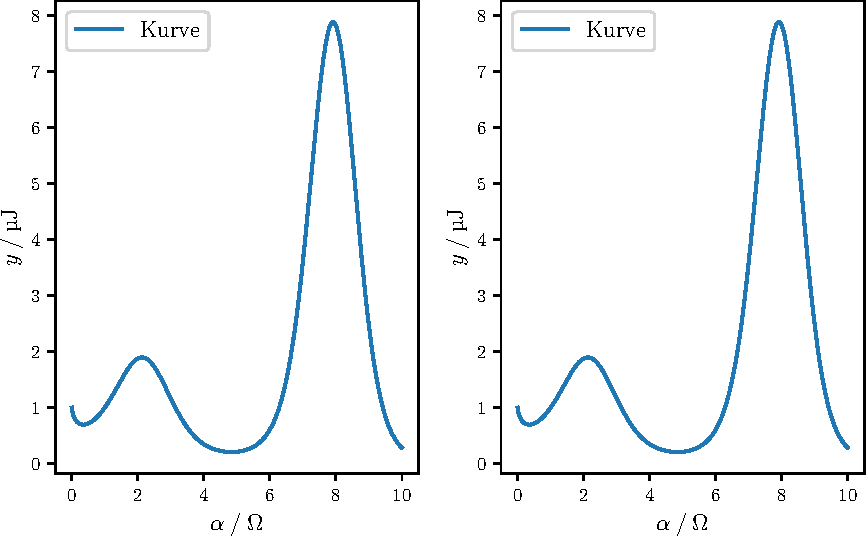
\includegraphics{build/plot.pdf}
    \caption{Filterkurve}
    \label{fig:filter}
\end{figure} 


